\documentclass[border=2pt]{standalone}
\usepackage{amsmath,amssymb}
\usepackage{diagrams}
\begin{document}
\begin{tikzpicture}[baseline=0pt, inner sep=0.1em,font=\scriptsize]
  % split the sign string (arg 10) and direction string (arg 11)
  \esplit{\signlst}{-+-+-+}%
  \esplit{\direcs}{ddddddddd}%
  % six hexagon vertices n0..n5 (n0 at the top, going counter-clockwise)
  \foreach \i in {0,...,5}{\coordinate (n\i) at (180+60*\i:0.8);}%
  % a signed dot at each vertex -- count from 0 so the index matches n\i
  \foreach \s [count=\i from 0] in \signlst {%
    \node[dotnode,label={180+60*\i:\vmksign{\s}}] at (n\i) {};%
  }%
  % stash each direction character in \dir0..\dir8 for per-slot testing.
  % \global because \foreach runs its body in a group.
  \foreach \d [count=\k from 0] in \direcs {%
    \global\expandafter\let\csname dir\k\endcsname\d}%
  % edges: fixed geometry per slot; \ifdir chooses forward vs reverse
  \ifdir{0}{\normedge{n0}{n1}{0.5}{-0.2}{$a$}}{\normedge{n1}{n0}{0.5}{0.2}{$a$}}%
  \ifdir{1}{\normedge[jmlinem=0.25]{n0}{n3}{0.25}{0.2}{$b$}}{\normedge[jmlinem=0.75]{n3}{n0}{0.75}{-0.2}{$b$}}%
  \ifdir{2}{\normedge{n0}{n5}{0.5}{0.2}{$c$}}{\normedge{n5}{n0}{0.5}{-0.2}{$c$}}%
  \ifdir{3}{\normedge{n2}{n1}{0.5}{0.2}{$g$}}{\normedge{n1}{n2}{0.5}{-0.2}{$g$}}%
  \ifdir{4}{\normedge{n2}{n3}{0.5}{-0.2}{$h$}}{\normedge{n3}{n2}{0.5}{0.2}{$h$}}%
  \ifdir{5}{\normedge[jmlinem=0.25]{n2}{n5}{0.25}{0.2}{$j$}}{\normedge[jmlinem=0.75]{n5}{n2}{0.75}{-0.2}{$j$}}%
  \ifdir{6}{\normedge[jmlinem=0.25]{n4}{n1}{0.25}{0.2}{$d$}}{\normedge[jmlinem=0.75]{n1}{n4}{0.75}{-0.2}{$d$}}%
  \ifdir{7}{\normedge{n4}{n3}{0.5}{0.2}{$e$}}{\normedge{n3}{n4}{0.5}{-0.2}{$e$}}%
  \ifdir{8}{\normedge{n4}{n5}{0.5}{-0.2}{$f$}}{\normedge{n5}{n4}{0.5}{0.2}{$f$}}%
\end{tikzpicture}
\end{document}
